Well, that was certainly an election night! Voters in 25 of Ohio's 88
counties were numerous enough to be \emph{more than one half of the
overall voters voting on the question} and caused Issue 1 to be passed.
The ``three C's'' (Cleveland, Columbus, and Cincinnati) plus Toledo and
Dayton as well as Painesville/Mentor, Chardon, Ashtabula, Athens,
Bowling Green, Youngstown, Cortland, and Put in Bay were all part of the
areas of the state that voted to pass this. Issue 1 will enshrine
abortion rights in the Ohio state constitution in roughly 30 days.

\begin{figure}
\centering
\pandocbounded{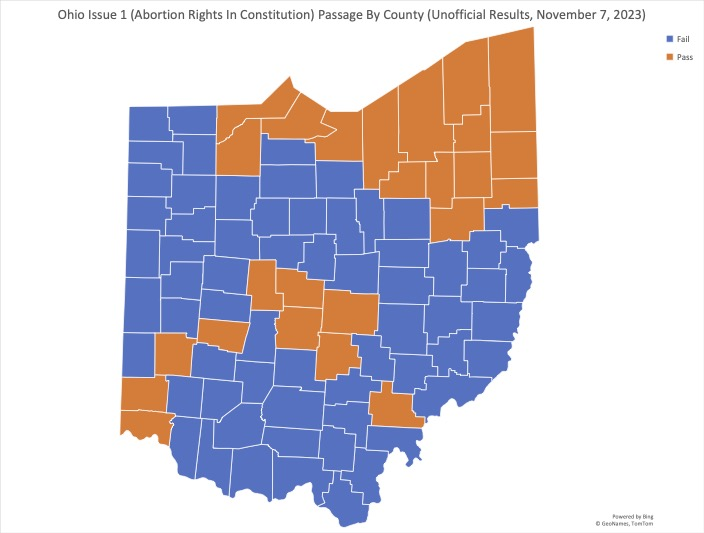
\includegraphics[keepaspectratio]{\%7B\%7Bsite.url\%7D\%7D/img/issue1passage.jpg}}
\caption{Graphic created using Microsoft Excel to illustrate passage by
county}
\end{figure}

It is a pity that this probably didn't settle anything at all. Julie
Carr Smyth had an interesting report run by the Associated Press linked
\href{https://web.archive.org/web/20231108033900/https://apnews.com/article/ohio-abortion-amendment-election-2023-fe3e06747b616507d8ca21ea26485270}{here}.
Here's the part that bothers me:

\begin{quote}
\emph{Republicans remained defiant in the wake of Tuesday's vote. Ohio
House Speaker Jason Stephens said Issue 1's approval ``is not the end of
the conversation.''}
\end{quote}

\begin{quote}
\emph{``As a 100\% pro-life conservative, I remain steadfastly committed
to protecting life, and that commitment is unwavering,'' Stephens said.
``The Legislature has multiple paths that we will explore to continue to
protect innocent life.''}
\end{quote}

\begin{quote}
\emph{Previously, state Senate President Matt Huffman, a Republican, has
suggested that lawmakers could come back with another proposed amendment
next year that would undo Issue 1, although they would have only a
six-week window after Election Day to get it on the 2024 primary
ballot.}
\end{quote}

We are a ``Super Tuesday'' state so this very well could come back to
haunt us in March during the presidential primary. If it does there
might well be some havoc. After almost a full year being overwhelmed
with this issue and facing the special election in August that tried to
derail this effort I think voters would move hard to punish legislators
if they pushed an immediate repeal attempt.

There are some weird costs to living in this state\ldots{}
